% The PGC Editor warm pipeline — internal engineering article.
% Companion to "The eventually consistent page" (TUGboat draft); same
% conventions, aimed at the product team and architects.
\documentclass{ltugboat}
\usepackage{microtype}
\usepackage{graphicx}
\usepackage{booktabs}
\usepackage{tikz}
\usetikzlibrary{arrows.meta, positioning, shapes.geometric, fit}
\usepackage[hidelinks,pdfa]{hyperref}

\def\LuaTeX{Lua\TeX}
\def\LuaLaTeX{Lua\LaTeX}
\setlength{\emergencystretch}{1.5em}

\title{The warm pipeline:\\ engine-resident recompilation\\ in the PGC Editor}
\author{Srikanth Mohankumar}
\address{TNQ Tech, Chennai, India}
\netaddress{srikanth.mohan (at) tnqtech dot com}

\begin{document}
\maketitle

\begin{abstract}
The PGC Editor compiles every correction through a full
XML\,$\to$\,\TeX\,$\to$\,PDF pipeline. Until recently each pass cost
18--25 seconds, almost all of it spent re-doing work that had not
changed: re-parsing conversion templates, re-loading the \TeX{}
template preamble, and re-typesetting every untouched paragraph. This
article describes the warm pipeline that replaces those repeated cold
starts with \emph{resident processes}: a persistent conversion worker,
a pool of preamble-resident \LuaTeX{} engines that accept a document
body over a pipe, and per-article \emph{serve} engines that re-typeset a
single paragraph in milliseconds and draw it live over the PDF as the
operator types. Builds now take 3--5 seconds with byte-verified
identical output, and a keystroke previews in about 0.2 seconds.
We explain how the \LuaTeX{} wrappers work, why the build engines are
single-shot while the preview engines are multi-shot, how paragraph
identity and typesetting context are captured, what the browser does
with the result, and how the system behaves when many operators work on
many articles at once. The companion research
article~\cite{srik:eventually} covers the underlying theory; this one
covers the production system.
\end{abstract}

\section{The problem, in numbers}

The PGC Editor is an XML-first correction tool: operators edit journal
XML in the browser, and every build converts XML to \TeX{} (the
\textsf{xml2tex} Node toolchain), compiles the \TeX{} with \LuaLaTeX{}
under the customer's production template, and returns the PDF. The
pipeline is correct and battle-tested --- and, before this work, it was
also completely stateless. Every build paid:

\begin{itemize}
\item \textbf{Conversion toolchain start-up.} A fresh Node process
  parsed the conversion templates every time: 0.7--1.9\,s before the
  first byte of \TeX{} existed.
\item \textbf{The template preamble.} On a representative ten-page ACS
  article, 13.1\,s of an 18.2\,s compile --- 72\% --- was the preamble:
  OpenType font loading, package initialization, structure-tagging
  machinery. None of it depends on the document body.
\item \textbf{The whole body.} Every paragraph re-typeset, even when
  the edit moved one comma.
\item \textbf{Polling.} The browser discovered the finished PDF by
  asking every two seconds, adding up to 2\,s of pure latency.
\end{itemize}

An operator who fixes a hyphen waits exactly as long as one who
rewrites a section. The fix is not a faster compiler --- Knuth--Plass line
breaking~\cite{knuth:linebreak} needs microseconds per
paragraph~\cite{lode:realtime} --- but an architecture that stops
discarding state between builds.

\section{Design rules}

Five rules shaped everything below; they are worth stating first
because they answer most ``what happens when \ldots'' questions by
construction.

\begin{enumerate}
\item \textbf{Warm state is keyed per article, never per user or
  globally.} Operators on different articles share nothing warm.
\item \textbf{Warm state is disposable.} Engines, workspaces, and
  captures are caches over the file server, which remains the only
  source of truth. Killing any warm process costs one slower build,
  never data.
\item \textbf{The cold path is never removed.} Any warm-path miss or
  failure falls back to today's pipeline automatically; the worst case
  \emph{equals} current behavior.
\item \textbf{Output must be identical, and gated.} A golden
  comparison (equivalent \texttt{.tex}, identical PDF text) guards the
  feature flag per customer. Speed never trades against fidelity.
\item \textbf{Memory is bounded by counting processes, not by hope.}
  Every resident thing has a cap, an idle reaper, and lives inside an
  explicit container memory limit.
\end{enumerate}

\section{Architecture overview}

\begin{figure*}[tb]
\centering
\resizebox{\textwidth}{!}{% Figure 1 — PGC Editor warm-pipeline architecture (wide, two-column span)
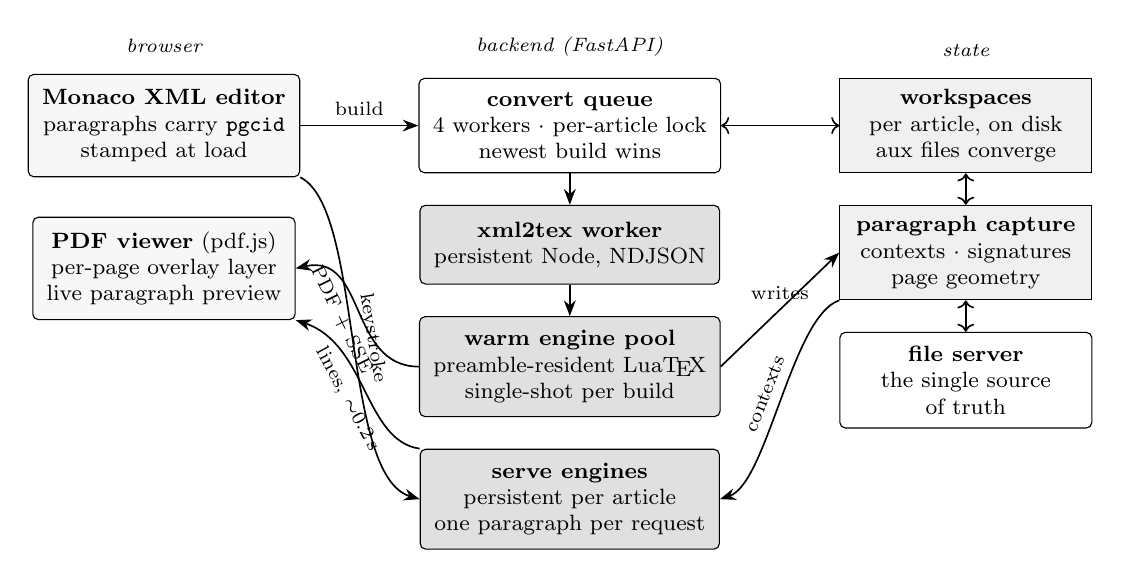
\begin{tikzpicture}[
  font=\footnotesize,
  box/.style={draw, rounded corners=2pt, align=center, inner sep=5pt,
              minimum height=8mm},
  store/.style={draw, align=center, inner sep=4pt, fill=black!6},
  eng/.style={box, fill=black!12},
  arr/.style={-{Stealth[length=2mm]}, semithick},
  node distance=6mm and 10mm]

  % browser column
  \node[box, fill=black!3, minimum width=32mm, minimum height=13mm]
    (editor) {\textbf{Monaco XML editor}\\ paragraphs carry \texttt{pgcid}\\ stamped at load};
  \node[box, fill=black!3, minimum width=32mm, minimum height=13mm, below=5mm of editor]
    (viewer) {\textbf{PDF viewer} (pdf.js)\\ per-page overlay layer\\ live paragraph preview};
  \node[font=\scriptsize\itshape, above=1.5mm of editor] {browser};

  % backend column
  \node[box, right=15mm of editor, minimum width=38mm, minimum height=11mm]
    (queue) {\textbf{convert queue}\\ 4 workers $\cdot$ per-article lock\\ newest build wins};
  \node[eng, below=4mm of queue, minimum width=38mm, minimum height=10mm]
    (x2t) {\textbf{xml2tex worker}\\ persistent Node, NDJSON};
  \node[eng, below=4mm of x2t, minimum width=38mm, minimum height=11mm]
    (pool) {\textbf{warm engine pool}\\ preamble-resident \LuaTeX\\ single-shot per build};
  \node[eng, below=4mm of pool, minimum width=38mm, minimum height=11mm]
    (serve) {\textbf{serve engines}\\ persistent per article\\ one paragraph per request};
  \node[font=\scriptsize\itshape, above=1.5mm of queue] {backend (FastAPI)};

  % state column
  \node[store, right=15mm of queue, minimum width=32mm, minimum height=10mm]
    (ws) {\textbf{workspaces}\\ per article, on disk\\ aux files converge};
  \node[store, below=4mm of ws, minimum width=32mm, minimum height=10mm]
    (cap) {\textbf{paragraph capture}\\ contexts $\cdot$ signatures\\ page geometry};
  \node[box, below=4mm of cap, minimum width=32mm, minimum height=10mm]
    (fs) {\textbf{file server}\\ the single source\\ of truth};
  \node[font=\scriptsize\itshape, above=1.5mm of ws] {state};

  % flows
  \draw[arr] (editor.east) -- node[above, font=\scriptsize]{build} (queue.west);
  \draw[arr] (editor.south east) .. controls +(8mm,-4mm) and +(-10mm,3mm) ..
    node[sloped, above, font=\scriptsize]{keystroke} (serve.west);
  \draw[arr] (queue) -- (x2t);
  \draw[arr] (x2t) -- (pool);
  \draw[arr] (pool.west) .. controls +(-9mm,0mm) and +(9mm,2mm) ..
    node[sloped, below, font=\scriptsize]{PDF + SSE} (viewer.east);
  \draw[arr] (serve.north west) .. controls +(-7mm,1mm) and +(9mm,-3mm) ..
    node[sloped, below, font=\scriptsize]{lines, $\sim$0.2\,s} (viewer.south east);
  \draw[arr] (pool.east) -- node[above, font=\scriptsize]{writes} (cap.west);
  \draw[arr, <->] (queue.east) -- (ws.west);
  \draw[arr, <->] (ws) -- (cap);
  \draw[arr, <->] (cap) -- (fs);
  \draw[arr] (cap.south west) .. controls +(-6mm,-2mm) and +(6mm,2mm) ..
    node[sloped, above, font=\scriptsize]{contexts} (serve.east);
\end{tikzpicture}
}
\caption{The warm pipeline. Two paths leave the editor: builds go
through the convert queue to a preamble-resident engine; keystrokes go
directly to the article's serve engine and return line data for the
viewer's overlay. Everything shaded is a resident process; everything
dashed-boxed is disposable per-article state over the file server.}
\label{fig:arch}
\end{figure*}

Figure~\ref{fig:arch} shows the system. The browser keeps its two
panes --- a Monaco XML editor and a pdf.js viewer --- but gains two
things: paragraphs carry a stable identity (\texttt{pgcid}), and the
viewer owns a per-page overlay layer. The backend gains three kinds of
resident process (conversion worker, warm build engines, serve
engines) and one kind of durable-ish state (per-article workspaces
holding converged aux files and the paragraph capture).

There are two request paths. A \emph{build} flows as today ---
queue, convert, compile, PDF --- except every stage is warm. A
\emph{keystroke} takes a much shorter path: resolve which paragraph the
cursor is in, re-typeset only that paragraph in the article's serve
engine, and draw the resulting lines over the stale PDF. The build path
produces truth; the keystroke path produces an exact preview of one
paragraph while truth is still being made.

\section{The \LuaTeX{} wrapper: anatomy of a warm engine}

The heart of the system is a small Lua harness that turns a normal
\texttt{lualatex} process into a server. The trick, shared with the
research prototype, is a \TeX-side loop:

\begin{verbatim}
\loop\directlua{ENGINE_ONE()}%
\ifserving\repeat
\end{verbatim}

The engine compiles the article's \emph{preamble} normally --- fonts,
packages, tagging machinery, everything up to
\verb|\begin{document}| --- and then enters that loop instead of
reading a body from the file. Each iteration calls a Lua function that
blocks on \texttt{stdin}. The protocol
(figure~\ref{fig:protocol}) is four lines long:

\begin{description}
\item[\texttt{ENGINEREADY}] emitted once, after the preamble has
  typeset. The pool now counts this engine as warm. Everything
  expensive has already happened.
\item[\texttt{RUN body.tex capture.json}] the pool asks for a build.
  The harness reads the body file and feeds it to \TeX{} with
  \texttt{tex.print}; \TeX{} typesets it exactly as if it had followed
  \verb|\begin{document}| in a normal run. The optional second
  argument enables paragraph capture (section~\ref{sec:capture}).
\item[\texttt{ENGINEDONE <ms>}] the body finished shipping pages;
  the elapsed body time is reported for telemetry.
\item[\texttt{QUIT}] the harness lets the loop fall through to
  \verb|\end{document}|. This is not process murder: the engine runs
  its normal shutdown, which is what writes the PDF cross-reference
  table and trailer. \emph{A killed engine leaves a truncated PDF; a
  quit engine leaves a valid one.}
\end{description}

\begin{figure}[tb]
\centering
\resizebox{\columnwidth}{!}{% Figure 2 — the warm engine wrapper protocol (column width)
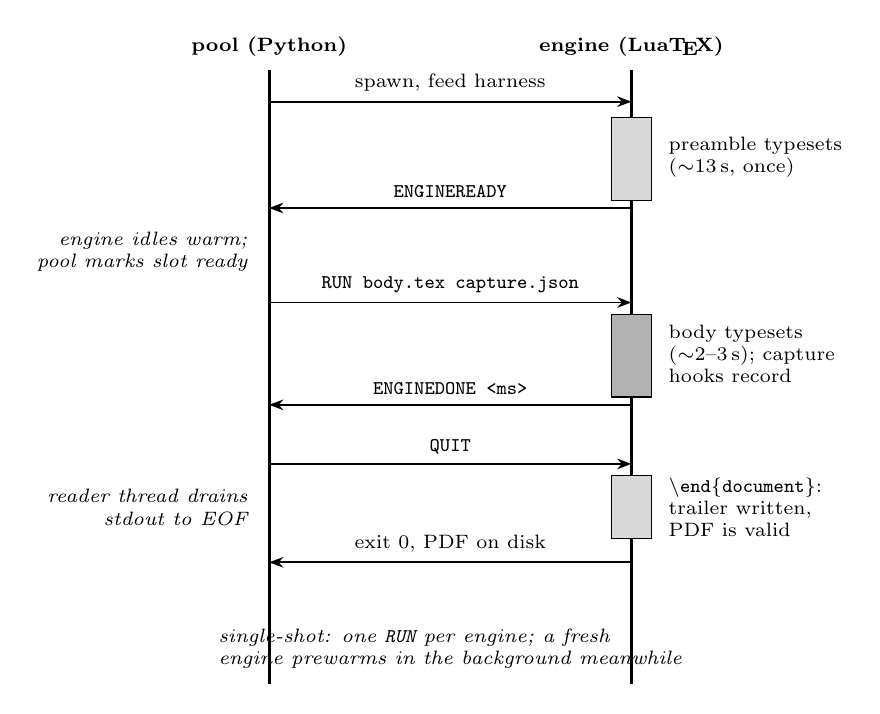
\begin{tikzpicture}[font=\scriptsize,
  msg/.style={-{Stealth[length=1.8mm]}, semithick},
  life/.style={very thick},
  ev/.style={font=\scriptsize\ttfamily}]

  % lifelines
  \node[font=\scriptsize\bfseries] (P0) at (0,6.4) {pool (Python)};
  \node[font=\scriptsize\bfseries] (E0) at (4.6,6.4) {engine (\LuaTeX)};
  \draw[life] (0,6.1) -- (0,-1.7);
  \draw[life] (4.6,6.1) -- (4.6,-1.7);

  \draw[msg] (0,5.7) -- node[above]{spawn, feed harness} (4.6,5.7);
  \draw[fill=black!15] (4.35,5.5) rectangle (4.85,4.45);
  \node[right, align=left] at (4.95,5.0)
    {preamble typesets\\ ($\sim$13\,s, once)};
  \draw[msg] (4.6,4.35) -- node[above, ev]{ENGINEREADY} (0,4.35);
  \node[left, align=right, font=\scriptsize\itshape] at (-0.15,3.8)
    {engine idles warm;\\ pool marks slot ready};

  \draw[msg] (0,3.15) -- node[above, ev]{RUN body.tex capture.json} (4.6,3.15);
  \draw[fill=black!30] (4.35,3.0) rectangle (4.85,1.95);
  \node[right, align=left] at (4.95,2.5)
    {body typesets\\ ($\sim$2--3\,s); capture\\ hooks record};
  \draw[msg] (4.6,1.85) -- node[above, ev]{ENGINEDONE <ms>} (0,1.85);

  \draw[msg] (0,1.1) -- node[above, ev]{QUIT} (4.6,1.1);
  \draw[fill=black!15] (4.35,0.95) rectangle (4.85,0.15);
  \node[right, align=left] at (4.95,0.55)
    {\texttt{\textbackslash end\{document\}}:\\ trailer written,\\ PDF is valid};
  \node[left, align=right, font=\scriptsize\itshape] at (-0.15,0.55)
    {reader thread drains\\ stdout to EOF};
  \draw[msg] (4.6,-0.15) -- node[above]{exit 0, PDF on disk} (0,-0.15);

  \node[align=left, font=\scriptsize\itshape] at (2.3,-1.25)
    {single-shot: one \texttt{RUN} per engine; a fresh\\
     engine prewarms in the background meanwhile};
\end{tikzpicture}
}
\caption{The warm-engine protocol. The preamble cost is paid before
\texttt{ENGINEREADY}; a build pays only the body. \texttt{QUIT} runs
the engine's normal shutdown so the PDF trailer is written.}
\label{fig:protocol}
\end{figure}

Two plumbing details cost us real debugging time and are worth
recording. First, \emph{somebody must drain the engine's stdout to
EOF}: \LuaTeX{} writes its log chatter to the pipe, and a full pipe
blocks the process --- including during the shutdown that finalizes
the PDF. Each engine gets a dedicated reader thread from birth to EOF.
Second, \LuaTeX's paranoid file-system setting
(\texttt{openout\_any=p}) silently rejects \emph{absolute} output
paths, so the capture file path is always passed relative to the
engine's working directory.

\subsection{Why build engines are single-shot}
\label{sec:singleshot}

The obvious design is one resident engine per article serving many
builds. We shipped the safe design instead: an engine serves exactly
one \texttt{RUN}, then quits, while a replacement prewarms in the
background. The reason is empirical. Production templates carry float
machinery, tagging state, and Lua-side bookkeeping that \emph{leak
across body re-runs}: in testing, the second body run through the same
engine silently lost figure pages. Snapshotting and restoring \TeX{}
registers was not sufficient --- the state lives partly in Lua tables
we do not own. Rather than chase every template's private state, we
guarantee first-run semantics by construction: every build is the
engine's first and only body. The output of a warm build was verified
byte-identical to a fresh cold compile before the flag ever turned on.

The cost of single-shot is hidden by \emph{prewarming}: a fresh engine
starts loading the preamble the moment an article is opened, and again
immediately after each build. The operator's next build almost always
finds a warm engine waiting. If it does not (first build after opening
a cold article), that build runs cold --- today's behavior --- while an
engine warms behind it.

\subsection{The pool}

The pool maps an article key (\texttt{customer/JIDaid}) to at most one
engine, holds at most \texttt{WARM\_MAX\_ENGINES} (default 6) engines
total, evicts least-recently-used when full, and reaps engines idle
longer than fifteen minutes. A pool miss is never an error --- it is a
cold build plus a background prewarm. The same shape applies to the
per-article workspaces on disk (capped at 50, reaped after 24 hours
idle): a workspace holds the article's converged aux files, so \TeX{}
cross-references are stable from the first warm build rather than
after two passes.

\section{The conversion worker}

The same resident-process treatment applies to XML\,$\to$\,\TeX.
A single persistent Node process loads the conversion machinery once
and serves conversions over a newline-delimited JSON pipe:
0.3--0.5\,s per conversion instead of 0.7--1.9\,s plus process spawn.
Because library code inside the worker may write to stdout, the worker
redirects console output to stderr and reserves stdout exclusively for
protocol frames; a single dedicated reader thread owns the pipe (two
readers on one pipe race and interleave), and the worker is recycled
automatically after a memory or request-count threshold, so a slow leak
in vendor code can never accumulate.

\section{Stable paragraph identity}

Everything per-paragraph depends on one invariant: a paragraph keeps
its identity across edits. The converter numbers paragraphs
(\texttt{pgcid}) idempotently --- ids present in the input XML are
preserved, and only unnumbered paragraphs receive fresh ids above the
maximum. We exploit this by stamping ids into the XML \emph{at load
time}, in the backend, before the operator ever sees the document.
The stamper is string-based --- it inserts attributes without
re-serializing the DOM, so untouched bytes stay untouched --- and its
output was proven identical to the converter's own numbering on
production articles (47/47 ids). The stamped file is persisted
atomically before it is served, so the editor, the converter, and the
capture all agree on identity from the first keystroke. On insertion
of a new paragraph, existing ids do not shift (0/46 shifted in
validation, against 39/46 with naive renumbering).

\section{Paragraph capture}
\label{sec:capture}

A warm build is also a measurement opportunity: the engine is
typesetting every paragraph anyway, so recording \emph{how} costs
almost nothing. When the pool passes a capture path with
\texttt{RUN}, the harness loads a capture module that hooks three
points in \LuaTeX's typesetting pipeline through its callback
interface~\cite{luatex:manual} --- the same mechanism packages such as
\textsf{lua-widow-control}~\cite{chernoff:lwc} use to manipulate
paragraphs at typesetting time:

\begin{description}
\item[Before line breaking] (\texttt{pre\_linebreak\_filter} together
  with the \texttt{insert\_local\_par} callback): record the paragraph's
  full line-breaking context --- about 25 parameters
  (\cs{hsize}, \cs{parindent}, \cs{tolerance}, penalties, demerits,
  \cs{baselineskip}, \cs{lineskip}, \cs{lineskiplimit}, language,
  microtype expansion state) plus the font in force at the paragraph's
  first glyph.
\item[After line breaking] (\texttt{post\_linebreak\_filter}): record
  the paragraph's \emph{line signature} --- per line, the height,
  depth, and every glyph with its exact horizontal position, measured
  with the engine's own arithmetic (\texttt{node.dimensions}), so
  microtype expansion is included to the scaled point.
\item[At shipout] (\texttt{pre\_shipout}): walk the finished page with
  absolute coordinates and record, per paragraph, its page number,
  origin, and bounding box. Vertical advance is accumulated as
  height-plus-depth of boxes and resolved glue --- never
  \texttt{node.dimensions} on a vertical list, which answers a
  different question.
\end{description}

Paragraphs are attributed to ids with a \TeX{} attribute set by the
\cs{paraid} markup the converter already emits. One production gotcha:
attributes are \emph{sticky}. Left alone after a paragraph ends, the
attribute bleeds into whatever the output routine contributes next ---
running heads and folios inherited the last paragraph's id and
corrupted its bounding box until the capture module explicitly resets
the attribute after each paragraph. The capture lands in the article's
workspace as JSON and is indexed in memory; because it lives in the
workspace, it survives backend restarts and is re-registered when the
article is next opened.

\section{The serve engine: one paragraph in milliseconds}

A preview request arrives with the operator's \emph{entire} current
XML, and the first thing the backend does is convert all of it --- through
the warm worker, so it costs 0.3--0.5\,s --- and then extract only the
edited paragraph's span from the resulting \TeX{} (located by the
\cs{paraid} wrapper the converter emits, sanitized against mid-edit
artifacts). Converting just the paragraph's XML in isolation would be
faster still, but the converter is document-scoped: numbering, counters,
cross-reference context and satellite-driven configuration all shape a
paragraph's \TeX{}. The preview's whole value is that its line breaks
are engine-exact, which requires the fragment's bytes to be identical
to a real build's --- so we keep the real converter on the real document
and make it resident instead of skipping it. (If previews ever need to
be faster, the lever is caching the conversion when nothing outside the
edited paragraph changed --- an optimization, not a redesign.)

The serve engine is the second kind of resident \LuaTeX{} process, and
it makes the opposite trade from the build engine. It is
\emph{multi-shot} --- one engine serves thousands of requests --- and
that is safe precisely because it never builds pages. Each request
typesets one paragraph inside

\begin{verbatim}
\setbox0=\vbox{<context><paragraph>\par}
\end{verbatim}

\noindent
and a box that is never shipped out engages no page builder, no float
placement, no output routine: none of the machinery that made build
engines leak (section~\ref{sec:singleshot}) ever runs. The request
prologue re-creates the captured context exactly --- all 25 parameters
and the start font --- so the line breaker sees the paragraph precisely
as the full build did. Cross-references and citations are transplanted
from the workspace's converged aux file directly into engine memory
(\texttt{token.set\_macro} on the \texttt{r@}/\texttt{b@} macros), so a
paragraph containing \cs{ref} or \cs{cite} resolves correctly without
ever loading the document. (Making cross-references single-pass by
construction is a related line of work; see
\textsf{monoref}~\cite{srik:monoref}.)

The response is the same line-signature JSON the capture produces,
which enables the key comparison: if the edited paragraph's
\emph{vertical profile} (per-line heights and depths, relative to the
first baseline) matches the captured one, the edit provably cannot move
anything else on any page --- the paragraph occupies exactly the same
vertical skeleton. The response carries a \texttt{profileChanged} flag
either way; the client shows the preview regardless and additionally
warns when the layout will shift on the next build.

Serve engines are per-article, capped (default 4) with LRU eviction and
an idle reaper, and are prewarmed at article open so the first
keystroke does not pay the spawn. Engine spawning happens outside the
registry lock (per-article spawn locks), so one article warming up
never blocks another article's preview. Measured on a production Sage
article: 164\,ms median end to end, with line breaks identical to the
full build to the scaled point.

\section{The frontend}

\begin{figure*}[tb]
\centering
\resizebox{\textwidth}{!}{% Figure 3 — the keystroke path, editor to overlay (wide)
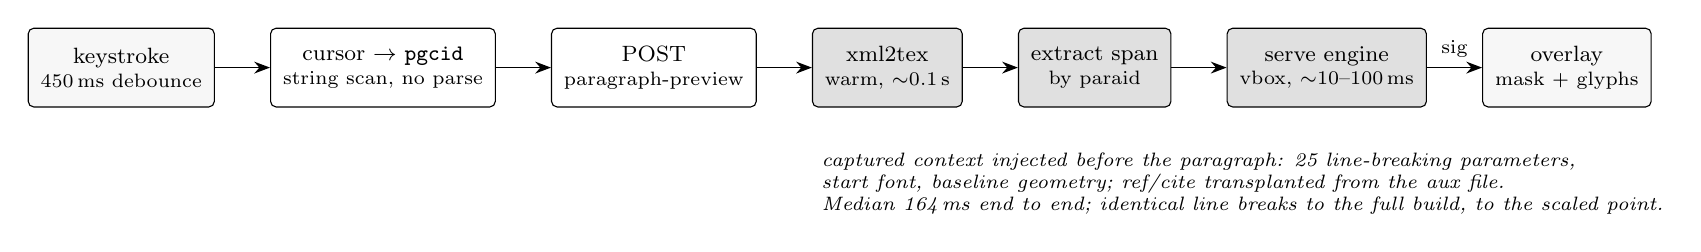
\begin{tikzpicture}[
  font=\footnotesize,
  stp/.style={draw, rounded corners=2pt, align=center, inner sep=4.5pt,
               minimum height=10mm},
  eng/.style={stp, fill=black!12},
  arr/.style={-{Stealth[length=2mm]}, semithick},
  node distance=5mm and 7mm]

  \node[stp, fill=black!3] (key) {keystroke\\[-1pt] {\scriptsize 450\,ms debounce}};
  \node[stp, right=of key] (para) {cursor $\to$ \texttt{pgcid}\\[-1pt]
    {\scriptsize string scan, no parse}};
  \node[stp, right=of para] (post) {POST\\[-1pt] {\scriptsize paragraph-preview}};
  \node[eng, right=of post] (x2t) {xml2tex\\[-1pt] {\scriptsize warm, $\sim$0.1\,s}};
  \node[eng, right=of x2t] (span) {extract span\\[-1pt]
    {\scriptsize by \cs{paraid}}};
  \node[eng, right=of span] (serve) {serve engine\\[-1pt]
    {\scriptsize \cs{vbox}, $\sim$10--100\,ms}};
  \node[stp, fill=black!3, right=of serve] (ovl) {overlay\\[-1pt]
    {\scriptsize mask + glyphs}};

  \draw[arr] (key) -- (para);
  \draw[arr] (para) -- (post);
  \draw[arr] (post) -- (x2t);
  \draw[arr] (x2t) -- (span);
  \draw[arr] (span) -- (serve);
  \draw[arr] (serve) -- node[above, font=\scriptsize]{sig} (ovl);

  \node[below=4.5mm of x2t.south west, anchor=north west, align=left,
        font=\scriptsize\itshape]
    {captured context injected before the paragraph: 25 line-breaking parameters,\\
     start font, baseline geometry; \cs{ref}/\cs{cite} transplanted from the aux file.\\
     Median 164\,ms end to end; identical line breaks to the full build, to the
     scaled point.};
\end{tikzpicture}
}
\caption{The keystroke path. Nothing here builds a page; the serve
engine re-typesets one paragraph in its captured context and the
browser draws the resulting glyphs over the stale PDF at their exact
positions.}
\label{fig:keystroke}
\end{figure*}

The browser closes the loop (figure~\ref{fig:keystroke}). On each XML
change, a 450\,ms debounce fires; at fire time --- not at
keystroke time --- the client resolves which paragraph encloses the
cursor with a dependency-free string scan of the XML (quote-aware,
skipping comments, CDATA, and processing instructions), so the preview
follows the operator even if they moved during the debounce. Requests
are single-flight: at most one preview is in the air, and a newer edit
re-resolves after the in-flight one settles rather than stacking.

The response is drawn into the PDF viewer's existing per-page overlay
slot: a near-opaque mask covers the paragraph's last-known extent
(from the captured bounding box), and the returned glyphs are placed
absolutely on top. Coordinates arrive in scaled points; the mapping is
$\mathrm{px} = \mathrm{sp}/65536 \times \mathrm{zoom}$, with the whole
paragraph anchored so its first glyph lands exactly on the captured
origin. The overlay is ephemeral by design: it clears the moment a
real build lands (the PDF underneath is now truth) or the operator
switches articles. If the backend reports the feature unavailable, the
client disables itself silently for the session --- the editor never
degrades below today's behavior.

Builds themselves also feel different: job completion is pushed over
server-sent events instead of discovered by polling, and if an
operator queues several builds only the newest compiles --- older
queued jobs return ``superseded'' without wasting an engine.

\section{Many operators, many articles}

\begin{figure}[tb]
\centering
% Figure 4 — per-article tenancy (column width)
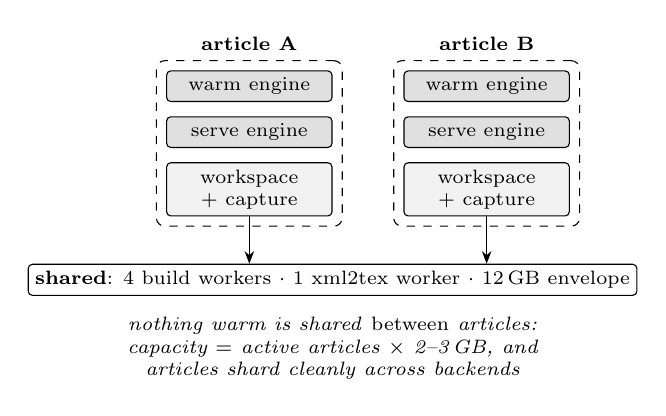
\begin{tikzpicture}[
  font=\scriptsize,
  lane/.style={draw, dashed, rounded corners=3pt, inner sep=3.5pt},
  cell/.style={draw, rounded corners=1.5pt, align=center, inner sep=2.5pt,
               minimum width=21mm, font=\scriptsize},
  hot/.style={cell, fill=black!12},
  st/.style={cell, fill=black!5},
  node distance=1.8mm and 4mm]

  % article A
  \node[hot] (a1) {warm engine};
  \node[hot, below=of a1] (a2) {serve engine};
  \node[st, below=of a2] (a3) {workspace\\ + capture};
  \node[lane, fit=(a1)(a2)(a3), label={[font=\scriptsize\bfseries]above:article A}] (A) {};

  % article B
  \node[hot, right=9mm of a1] (b1) {warm engine};
  \node[hot, below=of b1] (b2) {serve engine};
  \node[st, below=of b2] (b3) {workspace\\ + capture};
  \node[lane, fit=(b1)(b2)(b3), label={[font=\scriptsize\bfseries]above:article B}] (B) {};

  % shared band
  \node[cell, below=6mm of a3.south east, minimum width=47mm, anchor=north]
    (shared) {\textbf{shared}: 4 build workers $\cdot$ 1 xml2tex worker
      $\cdot$ 12\,GB envelope};

  \draw[-{Stealth[length=1.6mm]}] (a3.south) -- (shared.north -| a3.south);
  \draw[-{Stealth[length=1.6mm]}] (b3.south) -- (shared.north -| b3.south);

  \node[below=1.5mm of shared, align=center, font=\scriptsize\itshape]
    {nothing warm is shared \emph{between} articles:\\
     capacity $=$ active articles $\times$ 2--3\,GB, and\\
     articles shard cleanly across backends};
\end{tikzpicture}

\caption{Tenancy. Each article owns its warm set; only the build
workers, the conversion worker, and the memory envelope are shared.}
\label{fig:tenancy}
\end{figure}

Because all warm state is keyed per article
(figure~\ref{fig:tenancy}), the multi-user story reduces to a handful
of cases:

\begin{itemize}
\item \textbf{Different articles, simultaneous builds}: fully
  parallel up to the four build workers (unchanged from today), each
  against its own warm engine --- 3--5\,s each, no interaction.
\item \textbf{Same article, two operators}: the per-article lock
  serializes builds and supersession keeps only the newest --- the
  same single-owner model the editor has today, made fast.
\item \textbf{More open articles than warm slots}: LRU eviction; the
  evicted article's next build runs cold once while a fresh engine
  warms behind it.
\item \textbf{Idle or overnight}: reapers reclaim engine memory after
  fifteen minutes; the disk workspace survives 24 hours, so the next
  open prewarms straight back to warm.
\item \textbf{Crash, restart, out-of-memory kill}: warm state is
  disposable; captures re-register from the workspace at next open.
  One slower build, never data loss.
\end{itemize}

Capacity planning is therefore by \emph{article}, not by user: a fully
warm heavy-template article costs 2--3\,GB, and the default caps (6
build engines, 4 serve engines, 12\,GB container limit) are sized so
the worst case fits. Beyond one host, articles shard cleanly ---
sticky-route by article id, each backend owns its warm set, and the
shared file server remains the only truth.

\section{Correctness and limits}

The pipeline is flag-gated per environment and per customer
(\texttt{WARM\_ENGINES}), and the gate is empirical: an automated
golden comparison compiles the same article cold and warm and requires
an equivalent \texttt{.tex} (one known timestamp normalized) and
identical PDF text content. Fidelity of the paragraph fast path was
validated to \emph{zero scaled points} per glyph across four template
families in the research phase~\cite{srik:eventually}, and the
production battery (fourteen scenarios: parity, growth edits, hostile
mid-edit input, sequential load, engine-death recovery) passes 14/14.
The backend carries its first compile-path test suite (33 tests plus a
golden end-to-end test runnable against any dataset copy), and
\texttt{/metrics} exports per-stage warm/cold histograms; the
fallback-rate counter is the rollout health canary.

Known boundaries, by design rather than accident: paragraphs whose
typesetting depends on machinery a \cs{vbox} cannot reproduce ---
footnotes, display mathematics, list items, float captions (the wrapper
macro switches fonts mid-stream) --- are not eligible for the preview
fast path and simply take the 3--5\,s build path. The preview overlay
draws glyphs at engine-exact positions in the article's own typefaces,
fetched on demand through a font endpoint keyed by engine font id (a
serif fallback shows at the same positions until each face loads); the
next build still replaces the overlay with rendered truth.

\section{Measured results}

All figures below are from production articles on the development
host; ``cold'' is the pre-existing pipeline.

\begin{table}[hbt]
\centering
\small
\begin{tabular}{@{}lrrr@{}}
\toprule
Build & cold & warm & speedup\\
\midrule
ACS, 10\,pp, tagged      & 18.8\,s & 4.7\,s & 4.0$\times$\\
Sage, 14\,pp, floats     & 22.5\,s & 3.1\,s & 7.3$\times$\\
Live editor check        & 22.7\,s & 4.1\,s & 5.5$\times$\\
\bottomrule
\end{tabular}

\medskip

\begin{tabular}{@{}lr@{}}
\toprule
Keystroke path & latency\\
\midrule
preview, steady state (median)    & 164\,ms\\
first preview after article open  & $\sim$0.5\,s\\
same, without prewarm (hidden)    & $\sim$9\,s\\
conversion, warm worker           & 0.3--0.5\,s\\
\bottomrule
\end{tabular}
\caption{Measured build and keystroke latencies.}
\label{tab:results}
\end{table}

The qualitative change matters more than any single row of
table~\ref{tab:results}: checking a correction no longer requires a
build at all. The paragraph under the cursor updates in a fifth of a
second with engine-exact line breaks, the operator keeps typing, and
the 3--5\,s build --- when they ask for one --- confirms what the
overlay already showed.

\section{What is next}

Three threads continue. First, rendering images and rules inside the
preview region (the capture already records where they are). Second,
routing boundary paragraphs explicitly: the editor can know a cursor
is inside a footnote or display formula and say so, instead of
silently taking the slow path. Third, pushing background convergence
over the existing event stream, so the tiered model of the companion
article~\cite{srik:eventually} --- exact paragraph now, fresh pages in
seconds, true PDF shortly after --- is fully realized in the product.

\SetBibJustification{\raggedright}
\begin{thebibliography}{9}
\bibitem{knuth:linebreak}
Donald~E. Knuth and Michael~F. Plass.
\newblock Breaking paragraphs into lines.
\newblock \emph{Software: Practice and Experience}, 11(11):1119--1184,
  1981.

\bibitem{lode:realtime}
Clemens Lode.
\newblock Real-time \LuaTeX{}: Recompiling large documents in 1\,ms.
\newblock TUG 2026 preprint,
  \url{https://tug.org/tug2026/preprints/lode-realtime.pdf}, 2026.

\bibitem{luatex:manual}
The \LuaTeX{} development team.
\newblock \emph{\LuaTeX{} Reference Manual}, version 1.22.
\newblock \url{https://www.luatex.org/documentation.html}, 2025.

\bibitem{thanh:thesis}
Hàn Thế Thành.
\newblock \emph{Micro-typographic extensions to the \TeX{} typesetting
  system}.
\newblock PhD thesis, Masaryk University, Brno, 2000.

\bibitem{chernoff:lwc}
Max Chernoff.
\newblock Automatically removing widows and orphans with
  \textsf{lua-widow-control}.
\newblock \emph{TUGboat}, 43(1):28--39, 2022.

\bibitem{srik:monoref}
Srikanth Mohankumar.
\newblock \textsf{monoref}: single-pass cross-references for
  \LuaLaTeX{}.
\newblock CTAN, \url{https://ctan.org/pkg/monoref}, 2026.

\bibitem{srik:eventually}
Srikanth Mohankumar.
\newblock The eventually consistent page: tiered pagination for live
  \LuaLaTeX{} editing.
\newblock TUGboat article draft, TNQ Tech, 2026.
\end{thebibliography}

\makesignature
\end{document}
